\documentclass[preprint,12pt,sort&compress]{elsarticle}

\usepackage{amsmath}
\usepackage{booktabs}
\usepackage{graphicx}
\usepackage{lineno}
\usepackage{seqsplit}
\usepackage{url}

\journal{Applied Thermal Engineering}

\begin{document}

\begin{frontmatter}

\title{BubbleID-Flow: Reproducible Machine-Vision Quantification of Projected Vapor Coverage in Subcooled Flow Boiling}

\author[uark]{Abrar Fahim}
\author[cwru]{Farshad Barghi Golezani}
\author[uark]{Daniel Curl}
\author[uark]{Mohammad Ishraq Hossain}
\author[uark]{Stephen Pierson}
\author[cwru]{Chirag Kharangate}
\author[uark]{Han Hu\corref{cor1}}
\cortext[cor1]{Corresponding author.}
\ead{hanhu@uark.edu}

\address[uark]{Department of Mechanical Engineering, University of Arkansas, Fayetteville, AR, USA}
\address[cwru]{Department of Mechanical and Aerospace Engineering, Case Western Reserve University, Cleveland, OH, USA}

\begin{abstract}
Quantitative flow-boiling imaging requires segmentation accuracy, temporal dependence, and thermal provenance to be evaluated together. BubbleID-Flow applies one-class Detectron2 Mask R-CNN to 3000-fps images of subcooled FC-72 flow boiling in a 2.5 mm by 5.0 mm channel with a 114.6 mm heated length. The model was fine-tuned from 130 annotated images (104 training; 26 same-sequence holdout). On the holdout, its union mask achieved mean intersection over union of 0.652, Dice coefficient of 0.769, and projected-coverage mean absolute error of 0.0051, compared with 0.1891 for Otsu morphology and 0.0327 for a training-only Gaussian pixel classifier. The split is not independent: 25 of 26 holdout images have a training image within one source-sequence index, precluding experiment-level generalization and individual-bubble claims. Four complete 45 V sequences contained 88--108 frames. Circular moving-block bootstrap intervals were 2.0--3.6 times wider than independent-frame Student-$t$ intervals; effective sample sizes were 3.5--11.2. Recomputed sequence means differed from archived summaries by 0.00085 on average. Across 36 thermally matched states, projected coverage correlated with electrical heat flux within each case ($\rho_s=0.893$--1.000), but voltage and heat flux were perfectly rank-confounded. Adding coverage to a thermal baseline of heat flux, mass flux, and inlet subcooling did not improve leave-one-case-out prediction of seven-sensor surface temperature (RMSE: 6.92 versus 6.54 degC). The workflow therefore supports auditable two-dimensional projected coverage, not volumetric void fraction, universal regime criteria, or independently validated heat-transfer prediction.
\end{abstract}

\begin{keyword}
Flow boiling \sep Computer vision \sep Projected vapor coverage \sep Mask R-CNN \sep FC-72 \sep Temporal uncertainty \sep Reproducibility
\end{keyword}

\end{frontmatter}

\linenumbers

\section{Introduction}

Flow boiling supports high heat removal in compact thermal systems, but its performance depends on mass flux, inlet subcooling, geometry, heating configuration, and evolving liquid--vapor structure \cite{Mudawar2001,Mudawar2011,Kharangate2015,Shingote2024}. Thermal measurements provide heat input and surface response, whereas high-speed images expose the liquid--vapor structure that mediates wall rewetting, coalescence, and transport. Visualization has therefore long complemented thermal measurements: conventional image-processing studies have identified flow regimes, bubble size and growth, dryout-patch area and spreading, and projected vapor/void fraction from high-speed images \cite{Placzkowski2021Photographic,Li2021Visualization}. These observables are not interchangeable. A pixel-area ratio is a two-dimensional projected coverage unless channel depth, viewing geometry, and phase geometry are independently justified; it is not automatically a volumetric void fraction.

Machine vision now makes these measurements practical across image volumes that are prohibitively laborious to contour manually. U-Net-based methods have segmented subcooled-flow-boiling bubbles and combined masks with optical flow to estimate nucleation-site density, frequency, growth, sliding, and detachment quantities, with an independent infrared comparison in one facility \cite{Seong2023Automated}. Other flow-boiling workflows combine classical preprocessing or U-Net segmentation with flow-regime labels and image-derived void fractions \cite{Schepperle2024FlowRegimes}. Instance-segmentation and tracking pipelines extend the output from a union interface to bubble count, size, aspect ratio, wetting front, interfacial length, wavelength, vapor-layer thickness, and trajectories \cite{Chang2023BubbleMask,Huang2024BoilingPrediction}. General frameworks such as VISION-iT and BubbleID make explicit that detection, tracking, and post-processing are separate error sources, especially when occlusion, coalescence, morphology, illumination, heat flux, or surface condition change \cite{Suh2024VISIONiT,Dunlap2024BubbleID}.

This progress clarifies both the opportunity and the unresolved measurement burden. Learned masks can reduce manual processing and permit state-resolved descriptors, but they do not by themselves validate a physical quantity: overlapping vapor structures can defeat instance identities, clipped objects bias size statistics, adjacent frames are serially dependent, and random frame splits can overstate generalization. Further, a model trained for one image domain does not establish a three-dimensional void fraction, a universal regime threshold, or a causal optical--thermal relationship. Most directly relevant to the present facility, Naderi et al. analyzed 107 mini-channel flow-boiling cases and more than $3.8\times10^5$ images to connect spatial interfacial descriptors with heat-transfer prediction \cite{Naderi2026LargeScale}. That scale is appropriate for predictive generalization. The complementary need addressed here is a reproducible, small-data measurement chain that states what a flow-boiling image metric means, tests it against suitable baselines, quantifies temporal sampling uncertainty, and prevents optical--thermal or multimodal co-variation along an imposed ramp from being presented as independent evidence.

Three questions motivate this work. First, does the archived BubbleID-Flow checkpoint improve projected-coverage reconstruction relative to simple and learned pixel baselines? Second, how much does serial dependence among high-speed frames inflate uncertainty in a state mean? Third, does projected coverage add cross-condition information about the measured surface-temperature response beyond electrical heat flux, mass flux, and inlet subcooling? The resulting contribution is a reproducibility and claim-boundary study rather than a new heat-transfer correlation. Specifically, the paper (i) documents the annotation, model, inference, and combined-mask calculation; (ii) evaluates operating-point sensitivity, split leakage, and two baselines; (iii) replaces independent-frame confidence intervals with a moving-block bootstrap; (iv) audits the thermal source before testing incremental optical information; and (v) reports a timestamp-registered acoustic-emission state screen with its synchronization boundary. The deliberate primary output is union-mask projected vapor coverage, which remains meaningful when dense coalescence makes individual-bubble statistics fragile; the reproducibility artifacts preserve a path to add calibrated spatial profiles, interface measures, and validated tracking metrics rather than treating fine-tuning as the final scientific contribution.

\section{Experimental data}

\subsection{Flow loop and test section}

The data were collected during CWRU Test 17 on October 17, 2025. The working fluid was FC-72. The rectangular flow passage was 2.5 mm wide and 5.0 mm high, giving a cross-sectional area of $1.25\times10^{-5}$ m$^2$ and a hydraulic diameter of 3.33 mm. The bottom wall was electrically heated over a length of 114.6 mm, corresponding to a nominal heated area of $2.865\times10^{-4}$ m$^2$. Seven test-section surface-temperature locations were recorded at
\[
x=[0.0054,0.0227,0.0400,0.0573,0.0746,0.0919,0.1092]\ \mathrm{m}
\]
from the upstream end of the heated length. Figure~\ref{fig:facility} shows the loop, measurement streams, heated test section, and test matrix.

\begin{figure}[htbp]
  \centering
  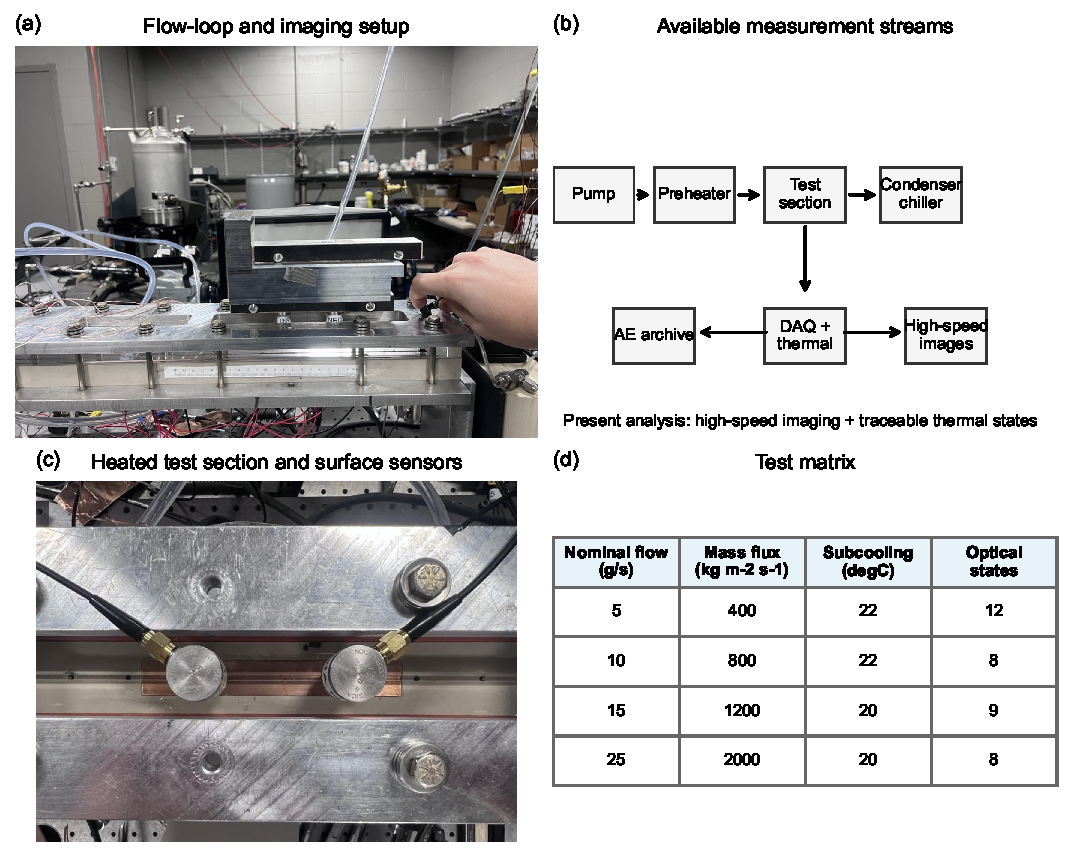
\includegraphics[width=\textwidth]{Figure_1_facility_data_streams.pdf}
  \caption{Facility and available data. (a) Flow-loop and imaging setup. (b) Loop and acquisition streams; the acoustic-emission archive supports timestamp-registered state screening only because common-trigger timing and sensor coupling are not verified. (c) Heated test section and surface-sensor access. (d) Nominal test matrix.}
  \label{fig:facility}
\end{figure}

The four image cases have nominal mass flow rates of 5, 10, 15, and 25 g/s and nominal inlet subcoolings of 22, 22, 20, and 20 degC, respectively. With the measured flow area, the matched thermal records give mean mass fluxes of approximately 395--443, 781--824, 1189--1209, and 1994--2010 kg m$^{-2}$ s$^{-1}$. Across the matched states, electrical heat flux spans 6.51--41.76 W cm$^{-2}$. Table~\ref{tab:test-matrix} identifies the available optical and thermal states.

\begin{table}[htbp]
  \centering
  \caption{Operating cases and auditable state coverage. One 10 g/s optical state at 45 V has no thermal row within the matching tolerance.}
  \label{tab:test-matrix}
  \begin{tabular}{lrrrr}
    \toprule
    Case & $\dot m$ (g/s) & $G$ (kg m$^{-2}$ s$^{-1}$) & Optical states & Matched states \\
    \midrule
    \texttt{5gs\_22C}  & 5  & 395--443   & 12 & 12 \\
    \texttt{10gs\_22C} & 10 & 781--824   & 8  & 7 \\
    \texttt{15gs\_20C} & 15 & 1189--1209 & 9  & 9 \\
    \texttt{25gs\_20C} & 25 & 1994--2010 & 8  & 8 \\
    \bottomrule
  \end{tabular}
\end{table}

Folder names combine applied voltage with operator labels such as onset or CHF. No objective onset, wall-dryout, or critical-heat-flux criterion was found in the supplied test notes. These labels are therefore retained only as archive identifiers. In the analysis and conclusions, the last folder in a sweep is called the operator-labeled endpoint; it is not treated as verified CHF.

\subsection{Optical and thermal records}

A FASTCAM SA-Z recorded 1024 by 1024 pixel images at 3000 frames/s. The model analyzes a fixed 1024 by 70 pixel near-wall region of interest (ROI) starting at image coordinate $(0,485)$. The pixel-to-length calibration and spatial registration between the ROI, heated surface, and seven temperature locations were not supplied. Accordingly, this paper reports neither dimensional bubble size nor local optical--thermal coupling.

The thermal workbooks contain time, mass flow, voltage, electrical power, inlet subcooling, inlet and outlet temperature, pressure, and seven test-section surface-temperature streams. Instrument model numbers, calibration records, heat-loss characterization, and sensor uncertainty were not available. Scatter within a selected time window is consequently reported as temporal variability, not as measurement uncertainty.

The archive also contains two-channel EasyAE acoustic-emission (AE) records: event-level HIT exports, 10 ms continuous TIME exports, and binary waveform-stream (WFS) files. The event and continuous streams use a 38 dBAE threshold. Archive notes place the sensors approximately at 25\% and 75\% of the heated length, but also identify mounting adequacy as a concern. These files enable a limited multimodal screening below; they do not provide a verified common trigger with the thermal or image acquisitions.

\section{Methods}

\subsection{Annotation, fine-tuning, and inference}

The annotation dataset contains 130 images and 130 Labelme JSON files. The labels \texttt{bubble} and \texttt{bubble\_cluster} are intentionally merged into one vapor-region category because the archived checkpoint is not a validated morphology classifier. Every fifth sorted image was assigned to the holdout, giving 104 training images with 7273 retained ROI annotations and 26 holdout images with 1908 annotations. Figure~\ref{fig:dataset-pipeline} summarizes the conversion to one-class COCO data.

\begin{figure}[htbp]
  \centering
  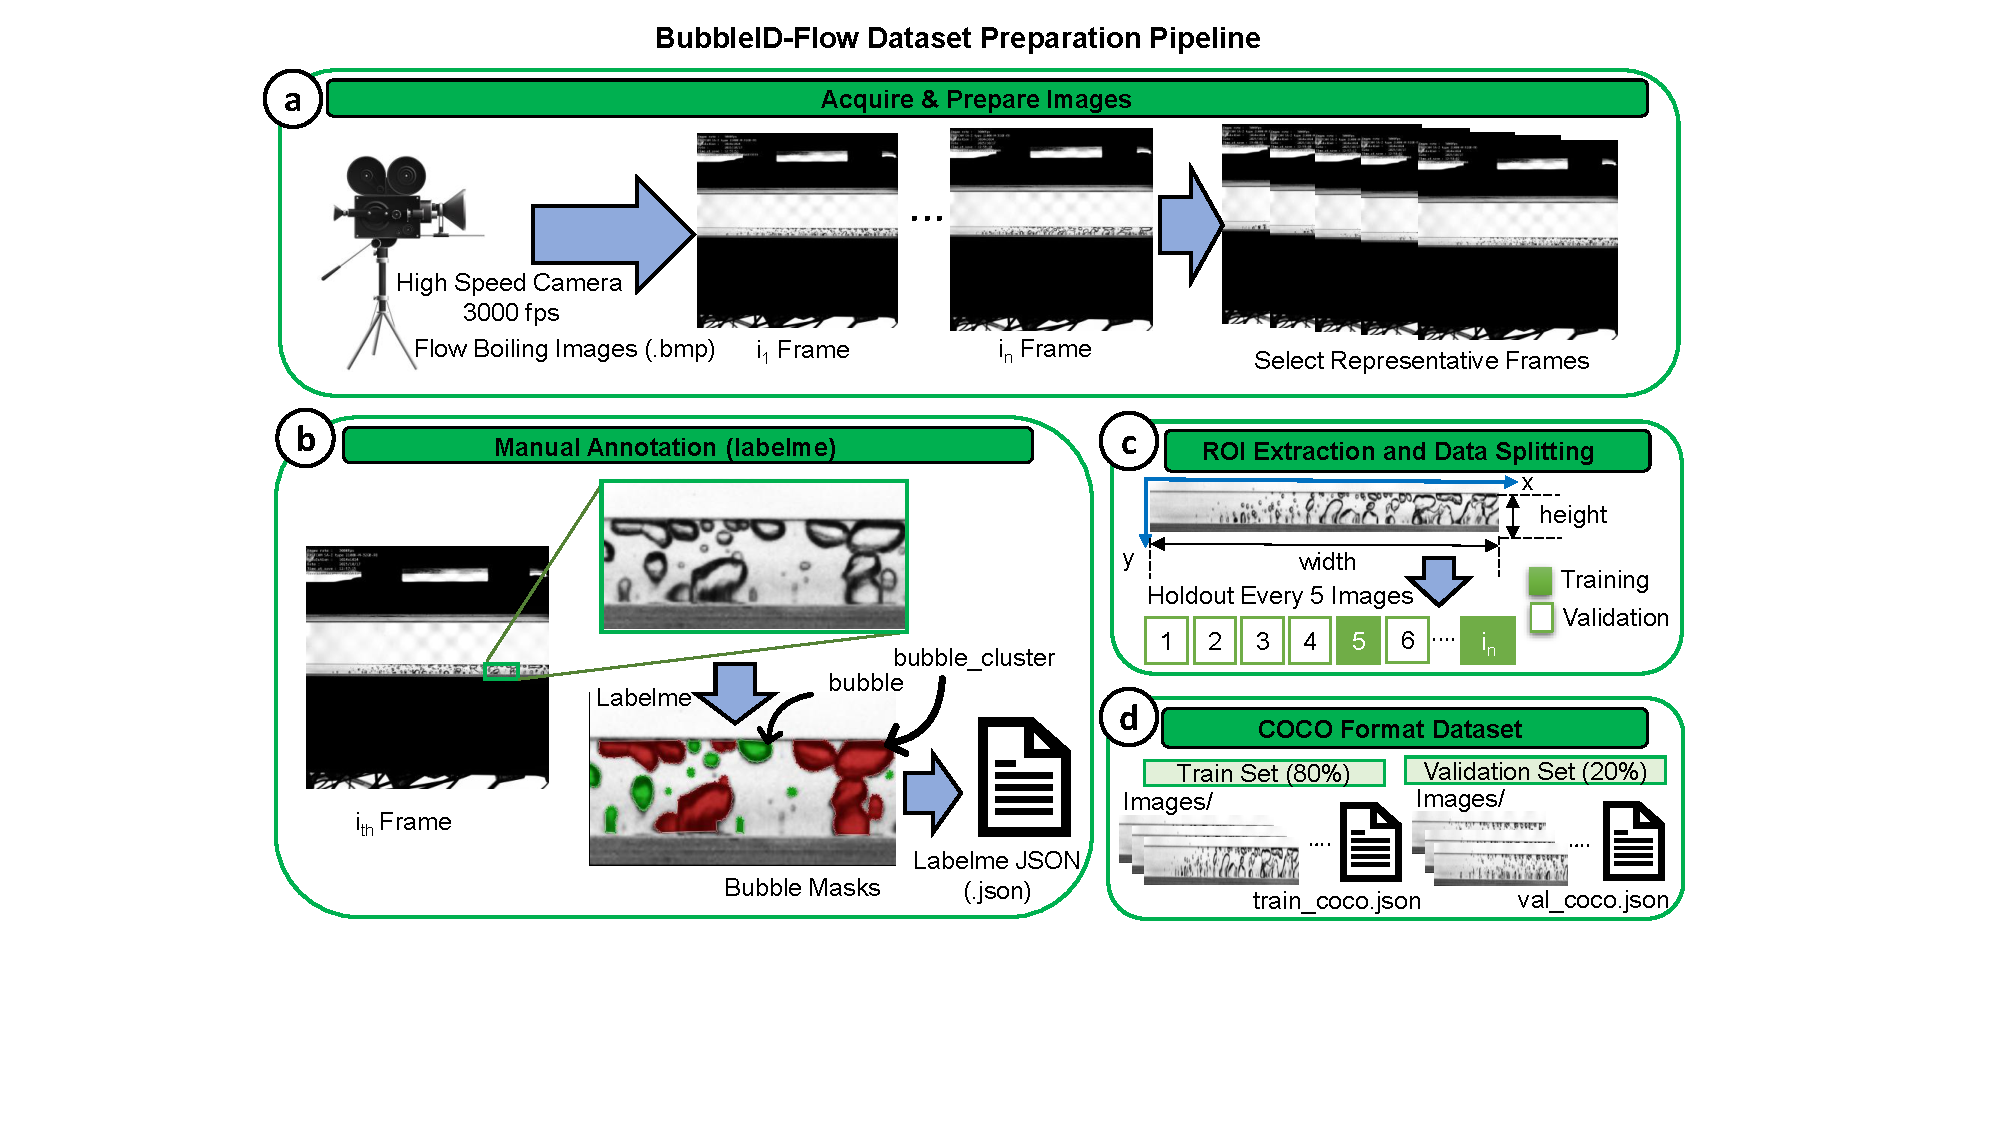
\includegraphics[width=\textwidth]{Figure_2_dataset_preparation_pipeline.pdf}
  \caption{Dataset preparation from high-speed frames and Labelme polygons to cropped, one-class COCO training and same-sequence holdout sets. This project-team schematic is used directly from the updated model package.}
  \label{fig:dataset-pipeline}
\end{figure}

The Detectron2 Mask R-CNN model used a ResNet-50 feature-pyramid backbone \cite{He2017MaskRCNN,Wu2019Detectron2}. The archived configuration specifies 2000 iterations, evaluation every 500 iterations, one image per batch, a base learning rate of $2.5\times10^{-4}$, and anchor sizes of 8, 16, 32, 64, and 128 pixels. Figure~\ref{fig:finetuning} shows the retained model-artifact flow. The original training log, seed, augmentation trace, and checkpoint-selection record were not supplied, so this study evaluates the archived weights but does not claim to reproduce fine-tuning.

\begin{figure}[htbp]
  \centering
  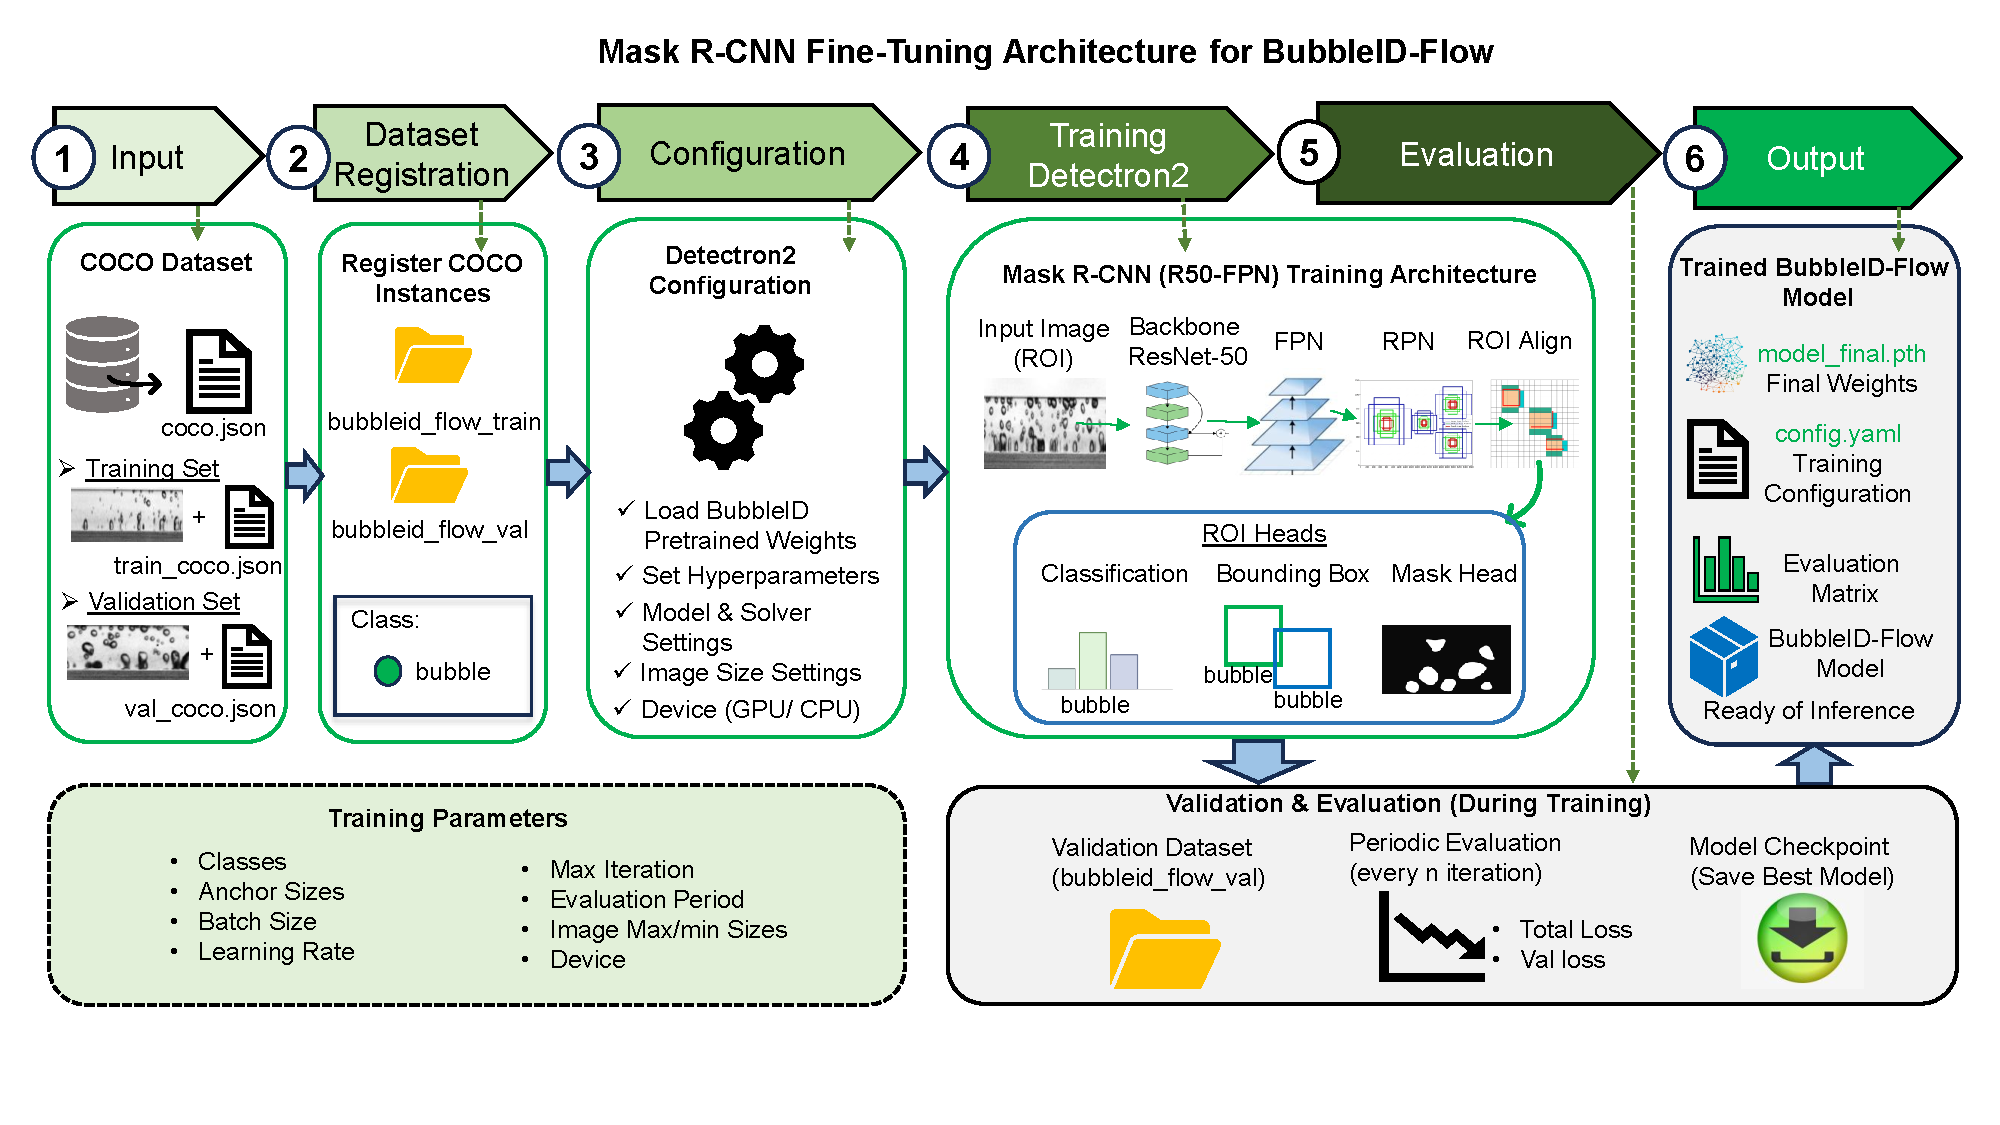
\includegraphics[width=\textwidth]{Figure_3_finetuning_architecture.pdf}
  \caption{Archived Mask R-CNN fine-tuning and inference workflow. This project-team schematic is used directly from the updated model package.}
  \label{fig:finetuning}
\end{figure}

The archived inference workflow prescribed a score threshold of 0.30 and at most 300 detections per image. All retained instance masks are combined before calculating projected vapor coverage,
\begin{equation}
\alpha_A=\frac{N_{\mathrm{vapor}}}{N_{\mathrm{ROI}}},
\label{eq:coverage}
\end{equation}
where $N_{\mathrm{vapor}}$ is the number of pixels in the union mask and $N_{\mathrm{ROI}}$ is the ROI pixel count. Thus $\alpha_A$ is a two-dimensional projected area fraction in the camera plane, not a volumetric void fraction.

Standard COCO metrics evaluate instance masks at a 0.05 score threshold. The engineering endpoint in Eq.~\eqref{eq:coverage} is evaluated at the archived 0.30 setting using union-mask IoU, Dice coefficient, signed coverage error, and absolute coverage error. A post hoc score-threshold sweep from 0.05 to 0.70 and detection-cap sweep from 50 to 300 assess sensitivity; they are not used as independent tuning evidence. Percentile intervals for image-level mean metrics use 10,000 deterministic bootstrap resamples. The split audit parses source-frame indices and computes nearest training--holdout proximity. Because all annotations derive from one source sequence, the holdout evaluates same-sequence reconstruction only.

\subsection{Segmentation baselines}

Two baselines test whether the deep model provides meaningful improvement. The fixed baseline applies grayscale Otsu thresholding followed by morphological cleanup, with no holdout tuning. The learned pixel baseline models vapor and background intensities with diagonal Gaussian likelihoods. Seventy-seven training images fit the class distributions; 27 sequence-grouped training images form a calibration subset for the probability threshold. Neither baseline uses the 26-image holdout for parameter selection. The same union-mask metrics are then evaluated on the holdout for all three methods.

\subsection{Temporal uncertainty}

Every available frame in the 45 V folder is processed for each case. Serial dependence is summarized by the integrated autocorrelation time
\begin{equation}
\tau_{\mathrm{int}}=1+2\sum_{k=1}^{K}\rho_k,
\qquad n_{\mathrm{eff}}=\frac{n}{\tau_{\mathrm{int}}},
\label{eq:tau}
\end{equation}
where the sum stops at the first non-positive autocorrelation in the initial positive sequence. Mean confidence intervals use a circular moving-block bootstrap with block length $\lceil\tau_{\mathrm{int}}\rceil$, 5000 resamples, and a fixed random seed \cite{Kunsch1989Bootstrap,Flyvbjerg1989Correlated}. Independent-frame Student-$t$ intervals are retained only as a diagnostic of underestimation.

\subsection{Traceable thermal reduction}

Only quantities recoverable from supplied measurements and documented geometry are used. Electrical heat flux and mass flux are
\begin{equation}
q''_e=\frac{P_e}{W L_h}, \qquad G=\frac{\dot m}{W H},
\label{eq:thermal}
\end{equation}
with $W=2.5$ mm, $H=5.0$ mm, and $L_h=114.6$ mm. The reconstructed $q''_e$ agrees with the workbook heat-flux column to numerical precision. For each voltage-labeled state, rows within $\pm0.75$ V are separated into contiguous blocks using a 5 s gap criterion; the largest non-overlapping block is retained. State means and standard deviations are then calculated for power, heat flux, mass flow, inlet and outlet temperatures, and the seven surface-temperature streams.

The source audit did not support use of the supplied heat-transfer coefficient, vapor quality, friction factor, or energy-balance columns. The archived reduction includes an undocumented multiplicative correction and unresolved unit and branch-logic ambiguities, while calibration, heat-loss, property-correlation, and uncertainty records are missing. Those derived quantities are therefore excluded rather than repaired through manuscript wording.

\subsection{Optical--thermal association test}

Spearman correlations between $q''_e$ and $\alpha_A$ describe each voltage sweep. Because applied voltage and heat flux are monotonic together, these correlations do not isolate an optical effect. Incremental information is tested with ridge regression for the mean of the seven measured surface temperatures, $\overline{T}_s$. The thermal baseline uses standardized $q''_e$, $G$, and inlet subcooling; the augmented model adds $\alpha_A$. Ridge strength is fixed at 1.0. Performance is calculated by leave-one-state-out and the stricter leave-one-case-out cross-validation. All preprocessing is fit within each training fold.

\subsection{Exploratory timestamp-registered acoustic screening}

The 10 g/s case was selected for a bounded acoustic screen because its seven thermally matched states have optical summaries, the AE HIT and TIME records span the thermal run, and the WFS stream covers the run. The thermal record started at 11:41:47.605 and the AE record at 11:42:13.000 on October 17, 2025, giving an archive timestamp offset of 25.395 s. Each thermal state interval was shifted by this offset to select an AE-relative window. This is timestamp registration, not a common hardware trigger or a synchronization validation.

For each registered interval and AE channel, we report vendor-defined continuous average signal level (ASL), HIT rate, and median HIT amplitude. Absolute-energy fields are retained only as vendor units in the reproducibility tables and are not interpreted as calibrated acoustic energy. The binary WFS file is decoded with the \texttt{decode-wfs} message format and count-to-voltage calibration using a bounded message-by-message reader \cite{Pierson2026DecodeWFS}; a 512-record prefix verifies two 1 MHz channels but is not state matched. The reusable parser and state-window implementation are retained in AELab \cite{UarkNed3AELab2026}. No acoustic regression, source localization, or causal optical--acoustic analysis is performed.

\section{Results and discussion}

\subsection{Checkpoint reconstruction and baseline comparison}

The same-sequence holdout gives bounding-box AP$_{50}=0.516$ and mask AP$_{50}=0.521$; AP averaged over IoU 0.50--0.95 is 0.234 for boxes and 0.249 for masks. At the archived 0.30 operating threshold, the combined masks give mean IoU 0.652, mean Dice 0.769, coverage MAE 0.0051, and mean signed error $+0.0021$. Bootstrap 95\% intervals are 0.573--0.721 for mean IoU, 0.690--0.830 for mean Dice, and 0.0037--0.0066 for mean absolute coverage error. Figure~\ref{fig:model-outputs} shows representative predictions.

\begin{figure}[htbp]
  \centering
  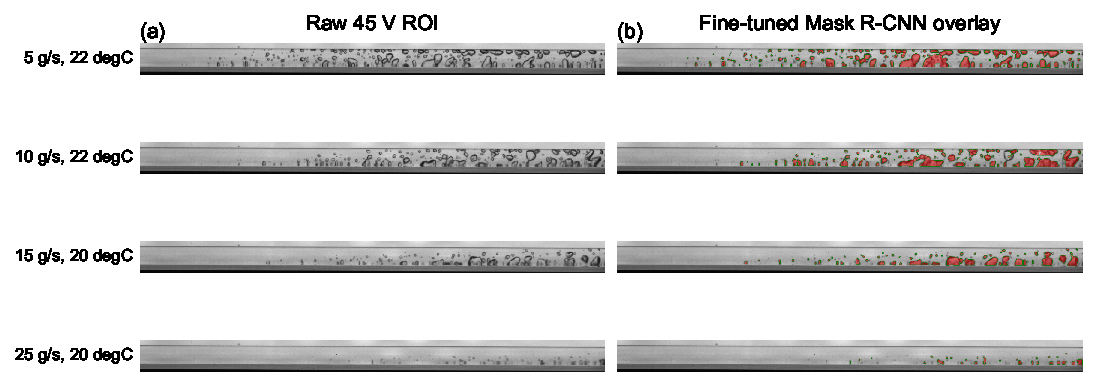
\includegraphics[width=\textwidth]{Figure_4_aug9_model_outputs.pdf}
  \caption{Representative 45 V near-wall ROIs for the four cases. Top: raw ROIs. Bottom: union-mask overlays from the archived one-class Mask R-CNN checkpoint at score threshold 0.30 and a 300-detection cap.}
  \label{fig:model-outputs}
\end{figure}

The error is coverage-dependent. Mean IoU is 0.444 for nine low-coverage images ($\alpha_A\leq0.05$), 0.758 for 13 intermediate images, and 0.775 for four high-coverage images. Low-coverage images have mean signed error $+0.0072$, whereas the high-coverage group has mean signed error $-0.0054$. Figure~\ref{fig:segmentation-robustness} also shows that overlap metrics peak at a different post hoc threshold than coverage MAE. A single operating point is therefore not a universal instance-segmentation optimum.

\begin{figure}[htbp]
  \centering
  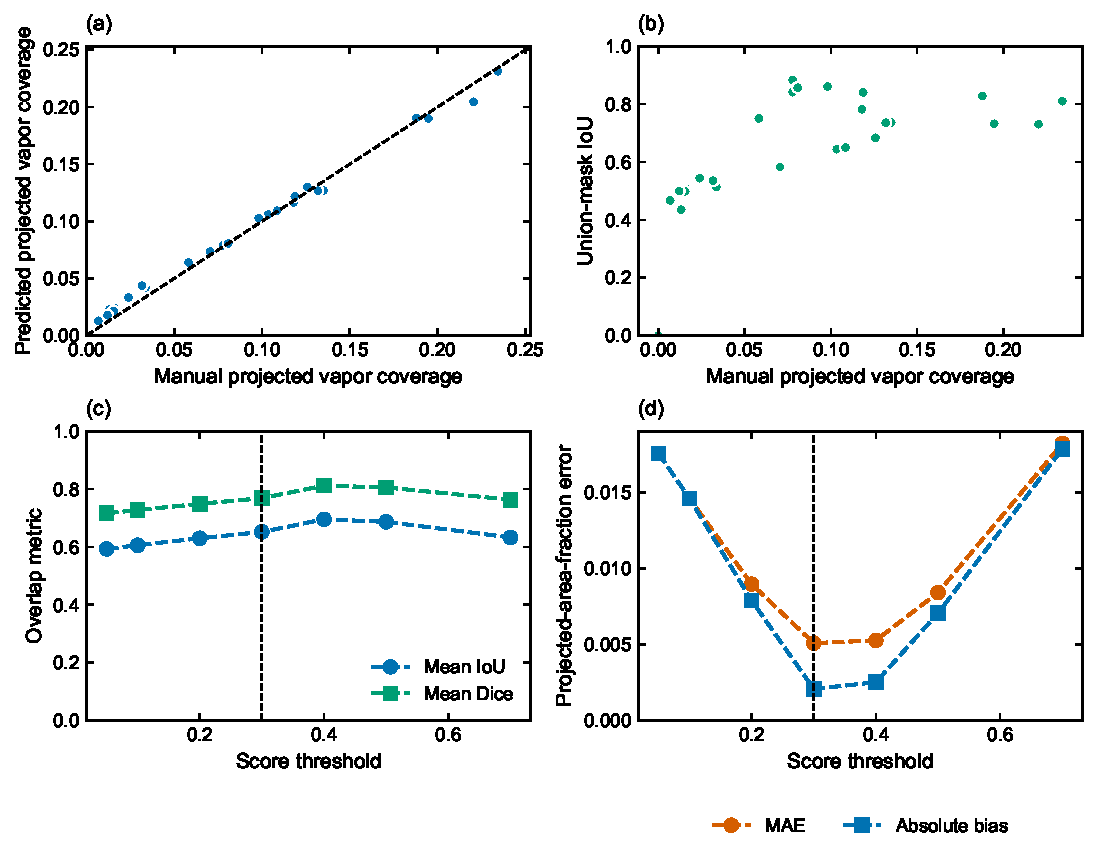
\includegraphics[width=0.93\textwidth]{Figure_5_segmentation_robustness.pdf}
  \caption{Same-sequence holdout sensitivity. (a) Predicted versus manual projected coverage. (b) Union-mask IoU versus manual coverage. (c) Mean IoU and Dice over score thresholds. (d) Coverage error over thresholds. Dashed vertical lines mark the archived 0.30 operating setting; the sweep is post hoc sensitivity analysis, not independent model selection.}
  \label{fig:segmentation-robustness}
\end{figure}

Table~\ref{tab:baselines} and Fig.~\ref{fig:baselines} show that Mask R-CNN substantially outperforms both baselines for coverage reconstruction. The Gaussian pixel classifier improves greatly over fixed Otsu morphology but still has 6.4 times the Mask R-CNN coverage MAE. This comparison supports the learned instance model for the stated union-coverage endpoint, while the modest instance AP continues to preclude reliable bubble counts and sizes.

\begin{table}[htbp]
  \centering
  \small
  \setlength{\tabcolsep}{5pt}
  \caption{Holdout segmentation comparison. The two baselines do not use holdout labels for parameter selection.}
  \label{tab:baselines}
  \begin{tabular}{lrrrr}
    \toprule
    Method & Mean IoU & Mean Dice & Coverage MAE & Signed error \\
    \midrule
    Otsu morphology & 0.209 & 0.331 & 0.1891 & $+0.1891$ \\
    Pixel Gaussian & 0.371 & 0.529 & 0.0327 & $+0.0258$ \\
    Mask R-CNN & 0.652 & 0.769 & 0.0051 & $+0.0021$ \\
    \bottomrule
  \end{tabular}
\end{table}

\begin{figure}[htbp]
  \centering
  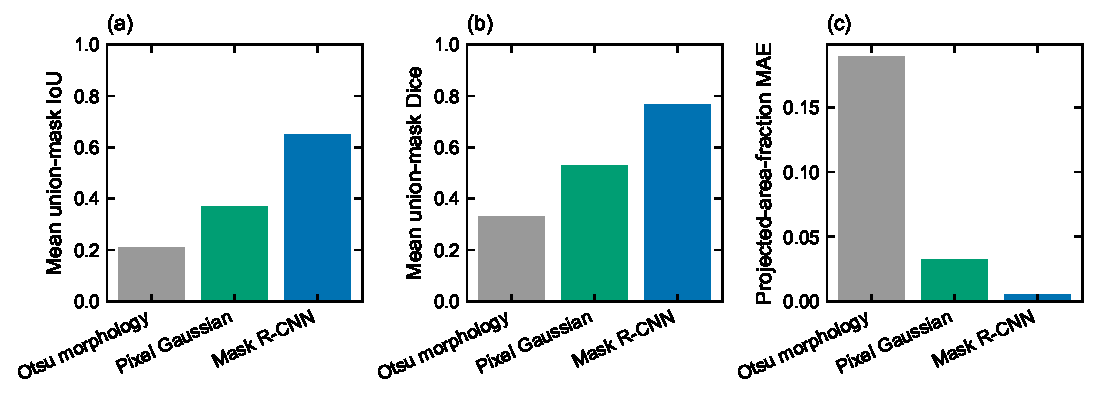
\includegraphics[width=0.95\textwidth]{Figure_6_segmentation_baselines.pdf}
  \caption{Simple and learned baseline evaluation on the 26-image holdout. (a) Predicted versus manual coverage. (b) Mean union-mask IoU and Dice. (c) Mean absolute coverage error. The Gaussian classifier is fit and calibrated using training images only.}
  \label{fig:baselines}
\end{figure}

The apparent strength of the aggregate metrics must be bounded by the split audit: ten holdout images share a nominal source-frame index with a training image through filename variants, and 25 of 26 have a training image within one source-sequence index. The evaluation therefore demonstrates same-sequence reconstruction, not robustness to a new run, camera, fluid, facility, or operating path.

\subsection{State trends and autocorrelation-aware uncertainty}

The archived 37-state summaries span $\alpha_A=0$--0.247. The 5 and 15 g/s sweeps increase to 0.247 and 0.190, respectively, over their recorded voltage folders. The 10 g/s sweep reaches 0.197 at 52.5 V and decreases to 0.076 in the final 55 V folder; the 25 g/s sweep reaches 0.113 at 57.5 V and decreases to 0.094 in the final 59 V folder. Because these endpoint folders lack an objective CHF criterion and most states lack regenerated frame-level outputs, the decreases cannot establish dryout or a universal transition threshold.

The four complete 45 V sequences contain 100, 108, 88, and 95 frames. Their recomputed means are 0.12897, 0.10882, 0.06556, and 0.01378, compared with archived values of 0.13086, 0.10966, 0.06536, and 0.01423. The four-case mean absolute difference is 0.00085. Table~\ref{tab:temporal} shows why treating frames as independent is inappropriate. Moving-block half-widths are 0.00103--0.00635, compared with 0.00044--0.00176 from Student-$t$ intervals.

\begin{table}[htbp]
  \centering
  \caption{Autocorrelation-aware uncertainty for complete 45 V sequences. CI denotes the 95\% moving-block-bootstrap interval.}
  \label{tab:temporal}
  \begin{tabular}{lrrrrr}
    \toprule
    Case & Frames & $\tau_{\mathrm{int}}$ & $n_{\mathrm{eff}}$ & Mean $\alpha_A$ & 95\% CI \\
    \midrule
    5 g/s  & 100 & 10.19 & 9.82 & 0.12897 & 0.12631--0.13190 \\
    10 g/s & 108 & 9.64  & 11.20 & 0.10882 & 0.10514--0.11255 \\
    15 g/s & 88  & 25.00 & 3.52 & 0.06556 & 0.05905--0.07175 \\
    25 g/s & 95  & 9.84  & 9.66 & 0.01378 & 0.01274--0.01481 \\
    \bottomrule
  \end{tabular}
\end{table}

\begin{figure}[htbp]
  \centering
  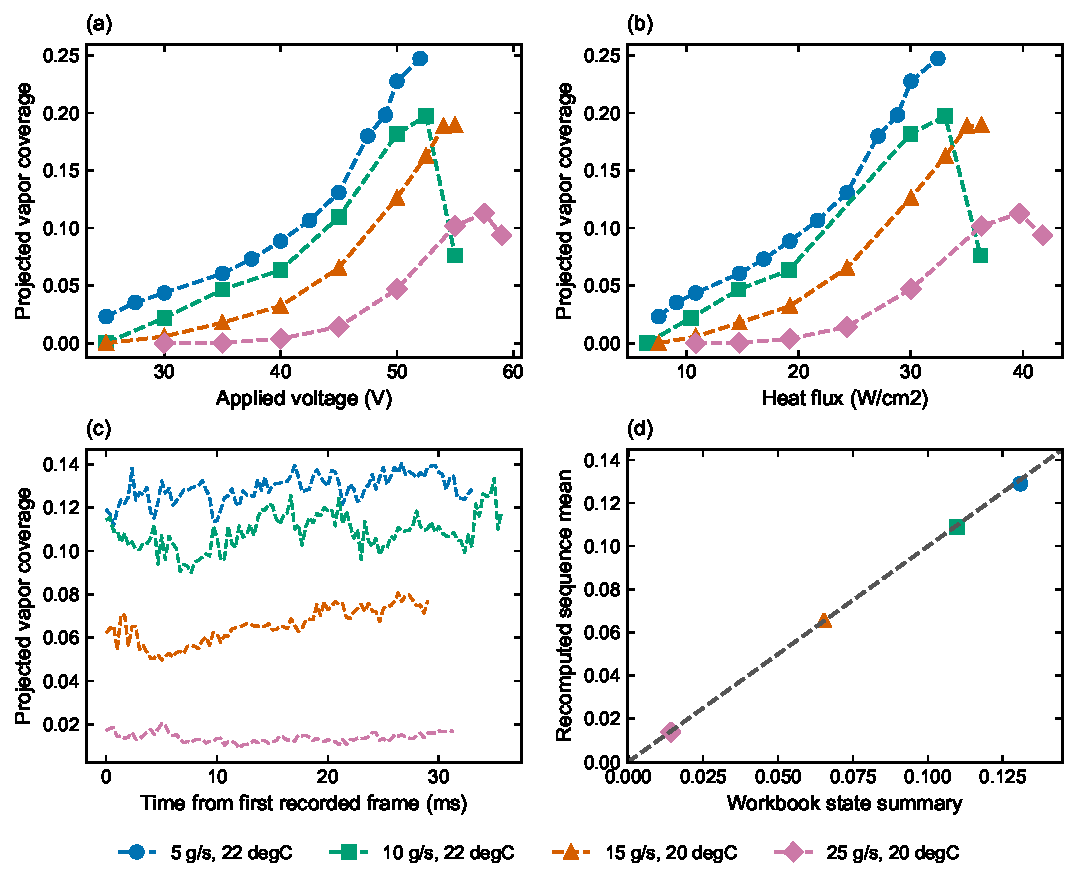
\includegraphics[width=\textwidth]{Figure_5_aug9_optical_results.pdf}
  \caption{Optical state and sequence results. (a) Archived projected-coverage summaries versus voltage. (b) Summaries versus matched electrical heat flux; the 10 g/s, 45 V point is omitted because no thermal window matched. (c) Every available frame in the four complete 45 V sequences. (d) Recomputed sequence means versus archived 45 V summaries. Autocorrelation-aware numerical intervals are reported in Table~\ref{tab:temporal}.}
  \label{fig:optical-results}
\end{figure}

Agreement at 45 V verifies the documented image-to-coverage implementation for a common state using the same checkpoint and source images. It is not independent model validation. The effective sample sizes also show that acquiring many adjacent frames does not provide the precision implied by the raw frame count.

The scope of the reported metric is intentional. Union-mask coverage is robust to the practical question of how much of the fixed image ROI is classified as vapor, whereas bubble count, equivalent diameter, aspect ratio, wetting-front length, and velocity require reliable instance separation, camera calibration, and temporal linking. The present holdout cannot validate those downstream quantities: its images are same-sequence, its instances have low AP, and the optical ROI is not registered to the heated surface. The repository therefore retains the masks and frame-level outputs needed for subsequent spatial-coverage and interface analyses, but it does not relabel projected coverage as volumetric void fraction or report unvalidated bubble-dynamics statistics.

A checkpointed all-state rerun also completed the 25, 27.5, and 30 V folders of the 5 g/s case before the CPU run was stopped. Their 88, 99, and 103 frame means are 0.02195, 0.03251, and 0.04138, differing from the archived summaries by $-0.00115$, $-0.00296$, and $-0.00234$. These differences are larger than two of the four 45 V differences and confirm that an archived state summary is not interchangeable with a complete-sequence mean. The partial three-state result is retained as provenance evidence but is not mixed into the cross-case figure.

\subsection{Thermal association and incremental information}

Within each voltage sweep, Spearman correlations between $q''_e$ and $\alpha_A$ are 1.000, 0.893, 1.000, and 0.929 for increasing nominal mass flow. However, voltage and $q''_e$ have $\rho_s=1.000$ in every case. The optical correlation is therefore inseparable from the imposed voltage progression in these data.

The cross-validated temperature test reinforces this limitation. For leave-one-state-out validation, the thermal baseline gives RMSE 4.84 degC and MAE 2.90 degC; adding $\alpha_A$ worsens them to 5.57 and 3.11 degC. For leave-one-case-out validation, baseline RMSE and MAE are 6.54 and 5.45 degC, compared with 6.92 and 5.49 degC after adding coverage. Figure~\ref{fig:thermal-association} shows the within-case correlations, confounding, and held-out predictions. The result does not imply that interfacial structure is thermally irrelevant. It shows that this projected ROI metric, sample size, and operating design do not demonstrate incremental predictive information beyond the three thermal-control variables.

\begin{figure}[htbp]
  \centering
  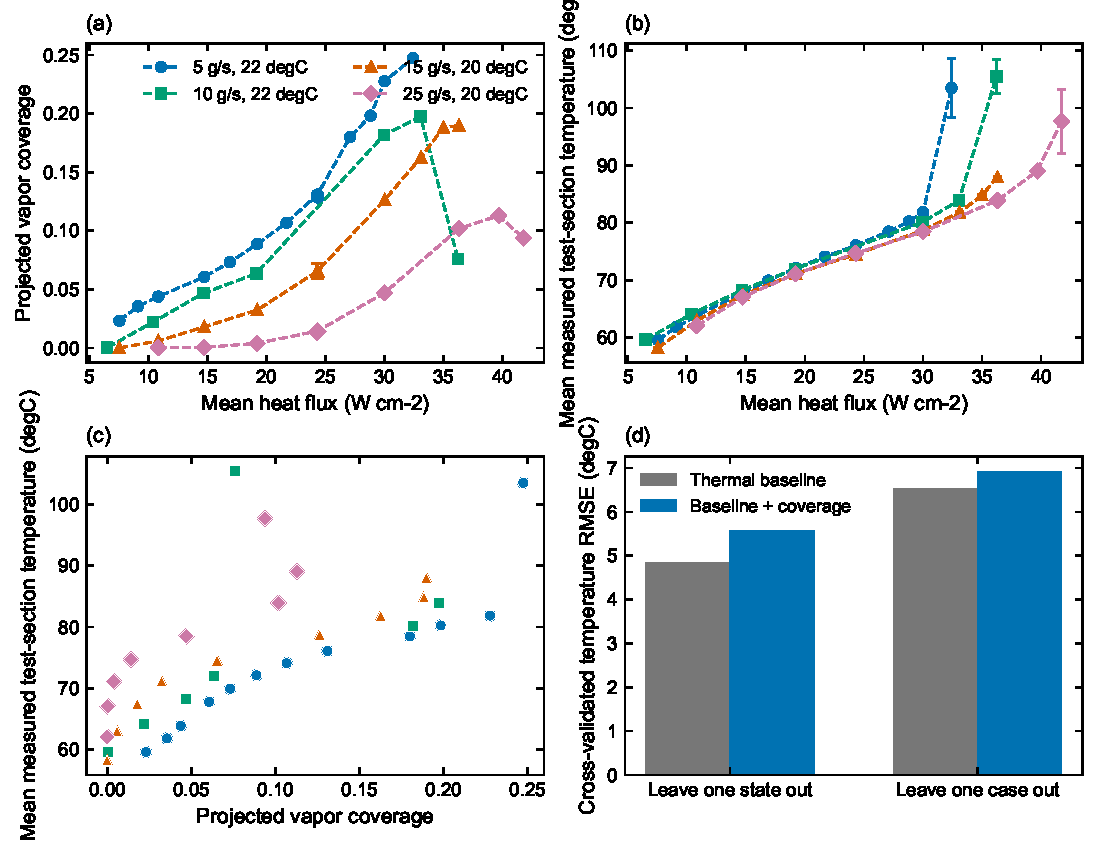
\includegraphics[width=\textwidth]{Figure_7_optical_thermal_association.pdf}
  \caption{Optical--thermal association audit for 36 matched states. (a) Projected coverage versus electrical heat flux; moving-block intervals are overlaid at the available 45 V states. (b) Mean seven-sensor surface temperature versus heat flux; error bars show the temporal standard deviation of the instantaneous seven-location average within each matched window. (c) Mean surface temperature versus projected coverage. (d) Cross-validated temperature RMSE for the thermal baseline and the baseline augmented with projected coverage.}
  \label{fig:thermal-association}
\end{figure}

\subsection{Timestamp-registered multimodal screening}

Figure~\ref{fig:multimodal-screening} summarizes the seven 10 g/s states with archive timestamp registration. Projected coverage increases from 0.00025 at 25 V to 0.197 at 52.5 V, then decreases to 0.076 in the final 55 V folder. Over the same imposed ramp, channel-1/channel-2 ASL increases from 24.38/23.38 dBAE to 35.49/37.61 dBAE and the corresponding event rates increase from 1.92/2.12 s$^{-1}$ to 928/638 s$^{-1}$. The terminal optical decrease while AE measures remain elevated is a useful diagnostic that a single projected ROI metric and an AE activity metric are not interchangeable state indicators.

However, all three modalities are conditioned on the same voltage ramp, the acoustic windows depend on separate-system timestamps, and the archive reports possible sensor-coupling limitations. The figure therefore documents an exploratory multimodal co-variation screen, not a correlation coefficient, time-resolved coupling, acoustic origin, or a flow-regime classifier.

\begin{figure}[htbp]
  \centering
  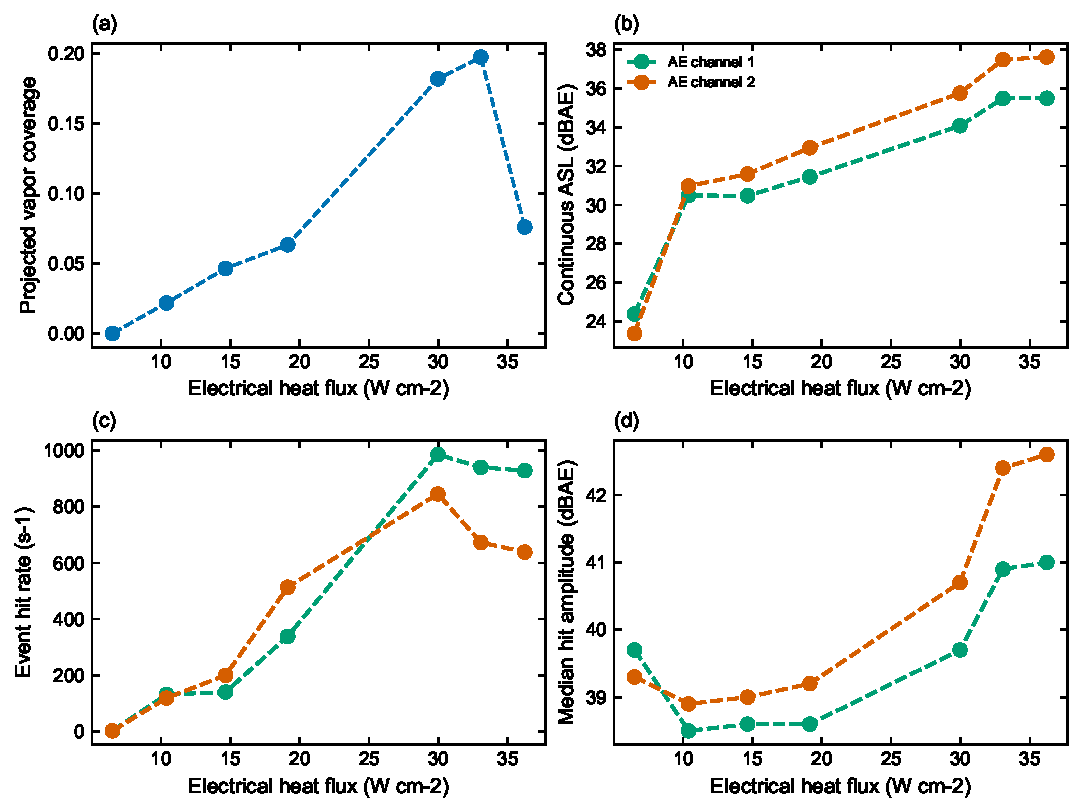
\includegraphics[width=\textwidth]{Figure_8_timestamp_registered_multimodal_screening.pdf}
  \caption{Exploratory 10 g/s multimodal state screen using archive timestamp registration. (a) Projected vapor coverage from the archived optical summary. (b) Continuous EasyAE average signal level. (c) Event hit rate. (d) Median event amplitude. Thermal state intervals are shifted by the 25.395 s difference between archive start timestamps. The records have no verified common trigger; lines show imposed-ramp co-variation only and do not establish optical--acoustic synchronization, causality, or source localization.}
  \label{fig:multimodal-screening}
\end{figure}

\section{Reproducibility, limitations, and required validation}

\begin{sloppypar}
The repository records the checkpoint SHA256, ROI, score threshold, detection cap, source hashes, generated CSV files, and deterministic analysis settings. The relevant entry points are \path{scripts/evaluate_detectron2.py}, \path{scripts/evaluate_segmentation_baselines.py}, \path{scripts/prepare_aug9_optical_results.py}, \path{scripts/audit_thermal_reduction.py}, and \path{scripts/analyze_optical_thermal_association.py}. The checkpoint SHA256 is \texttt{\seqsplit{6F60969CE876F57A78B53FC61895C99B92CB2E1B6F0E0B30F01FA301236042CD}}.
\end{sloppypar}

Five limitations define the present claim ceiling. First, the manual holdout is strongly dependent on the training sequence, and the 0.30 operating threshold has no experiment-independent calibration set. New manually annotated sequences held out by experiment and operating condition are required for generalization. Second, the four common 45 V folders and three additional low-voltage 5 g/s folders have complete regenerated frame outputs; 30 state values remain traceable derived summaries without complete-sequence temporal intervals. Third, the thermal records support electrical heat flux, mass flux, temperatures, and their within-window variability, but not a calibrated uncertainty budget or independently reproduced heat-transfer coefficient, quality, friction, or energy balance. Fourth, the optical ROI is not spatially registered to the heated surface or temperature locations and cannot measure three-dimensional void fraction. Fifth, the operator folder labels do not establish onset, CHF, or dryout. The 10 g/s acoustic screen is limited to timestamp-registered state summaries; a common trigger, quantified sensor coupling, calibration, and replicated runs are required before any quantitative optical--acoustic synchronization or inference claim.

These are not resolved by weaker wording alone. The next validation experiment should preserve trigger-synchronized image and thermal time bases; record instrument models, calibration, heat loss, and uncertainty; define onset and CHF independently from the images; collect replicate ramps; and reserve complete operating cases for annotation and blind evaluation. A calibrated view should then add streamwise coverage profiles and interface-length density before attempting instance tracks, diameters, or velocities; volumetric void fraction requires an explicit geometric or independent-reference validation. Until those data exist, BubbleID-Flow should be used as a traceable projected-coverage measurement within the present image domain.

\section{Conclusions}

\begin{sloppypar}
BubbleID-Flow provides a reproducible workflow for measuring two-dimensional projected vapor coverage from high-speed subcooled flow-boiling images while retaining the temporal, thermal, and acoustic provenance needed to constrain interpretation. On the 26-image same-sequence holdout, the archived Mask R-CNN checkpoint achieved union-mask IoU of 0.652, Dice coefficient of 0.769, and projected-coverage MAE of 0.0051, outperforming fixed Otsu and training-only Gaussian pixel baselines; however, the dependent split and mask AP of 0.249 do not support individual-bubble or experiment-level generalization. Complete 45 V sequences reproduced archived coverage means with a four-case MAE of 0.00085, while temporal autocorrelation reduced effective sample sizes to 3.5--11.2 and widened the corresponding mean intervals. Within each voltage sweep, projected coverage covaried with electrical heat flux, but the perfect rank association between voltage and heat flux prevents a separate optical effect from being identified, and coverage did not improve cross-validated prediction of mean measured surface temperature beyond heat flux, mass flux, and inlet subcooling. The timestamp-registered 10 g/s acoustic screen similarly documents imposed-ramp co-variation rather than trigger-synchronized or causal coupling. Thus, the present defensible contribution is an auditable projected-coverage measurement and a bounded multimodal screening workflow; volumetric void fraction, universal regime thresholds, CHF detection, calibrated heat-transfer prediction, and quantitative acoustic inference require independent validation.
\end{sloppypar}

\section*{CRediT authorship contribution statement}

Abrar Fahim: Data curation, Software, Formal analysis, Visualization, Writing -- review and editing. Farshad Barghi Golezani: Methodology, Software, Visualization, Formal analysis, Writing -- review and editing. Daniel Curl: Investigation, Data curation, Methodology, Validation. Mohammad Ishraq Hossain: Investigation, Data curation, Formal analysis, Writing -- original draft. Stephen Pierson: Contribution roles to be confirmed. Chirag Kharangate: Contribution roles to be confirmed. Han Hu: Conceptualization, Supervision, Funding acquisition, Project administration, Methodology, Writing -- review and editing. All roles require author confirmation before submission.

\section*{Declaration of competing interest}

The authors declare that they have no known competing financial interests or personal relationships that could have appeared to influence the work reported in this paper. All authors must confirm this statement before submission.

\section*{Funding}

This work was supported by the NSF/CASIS FBCE project and institutional research support. Grant numbers and sponsor roles remain to be verified before submission.

\section*{Data availability}

\begin{sloppypar}
Analysis code is available at \url{https://github.com/UARK-NED3/BubbleID-Flow}. The Aug. 9 fine-tuned Mask R-CNN weights are available through the OSF view-only record at \url{https://osf.io/xnkh6/overview?view_only=09d63d516ca0489e90fa9b94d37b529e}. The verified local checkpoint SHA256 is \texttt{\seqsplit{6F60969CE876F57A78B53FC61895C99B92CB2E1B6F0E0B30F01FA301236042CD}}. Raw optical and thermal records are maintained in the project archive but are not publicly released in the manuscript package; access remains subject to sponsor, collaborator, and institutional data-sharing approval.
\end{sloppypar}

\section*{Declaration of generative AI and AI-assisted technologies in the manuscript preparation process}

During preparation of this work, the authors used OpenAI Codex to assist with manuscript drafting, code organization, analysis scripts, and deterministic figure preparation. No generative image tool was used to create or alter the submitted scientific figures. The authors reviewed the resulting content and remain responsible for the manuscript.

\section*{Acknowledgments}

The authors acknowledge the CWRU experimental team for flow-loop access and data-collection support and the BubbleID and BubbleID-Flow contributors for software development. This statement should be finalized with all contributors before submission.

\bibliographystyle{elsarticle-num}
{\small
\bibliography{references}
}

\end{document}
